\chapter{Experiment Setup} \label{Chp: Experiment Setup}
%All experiments are done within the Cooja simulator. The environment we simulated is as described in \Cref{fig: Setup}.

In this chapter we describe how we set up our experiments. The related source code can be downloaded from: \url{https://github.com/Salties/MyRepository} .

\section{Overview}

\Cref{Fig: Experiment Setup} illustrates an overview of our experiment setup. 

\begin{figure*}[h!]
	\center
	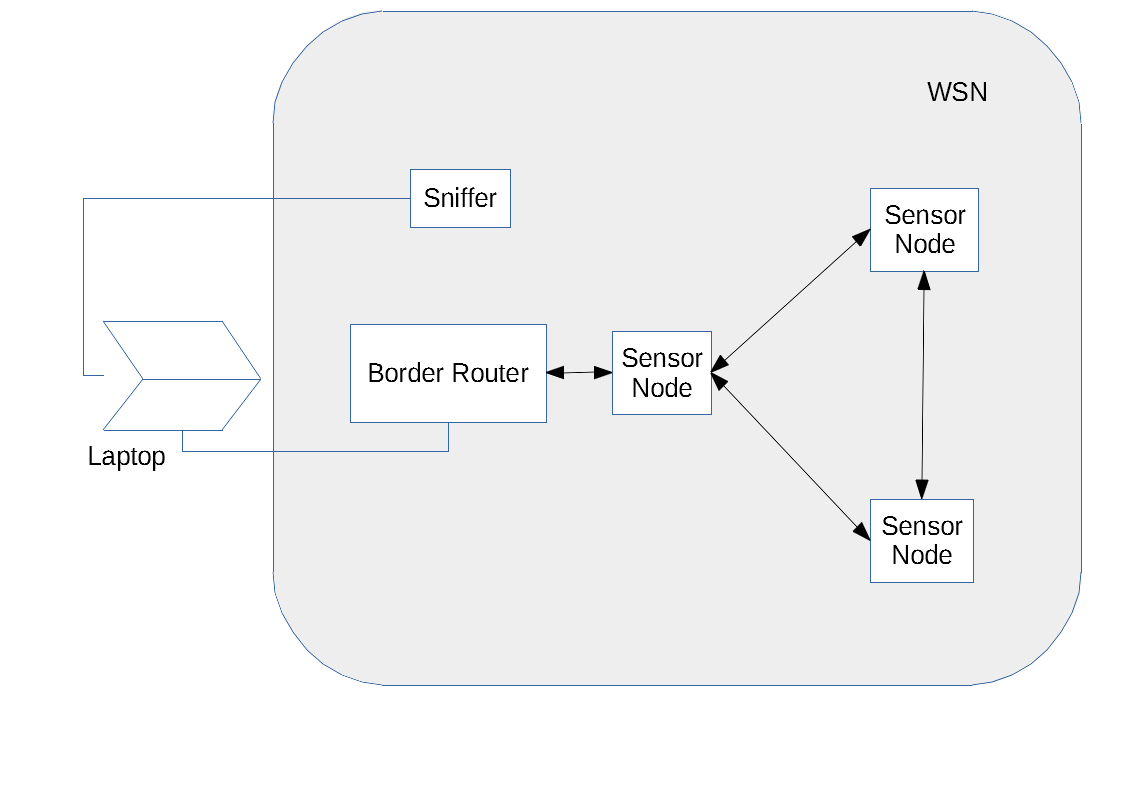
\includegraphics[width=0.75\textwidth,]{fig/setup.png}
	\caption{Experiment Setup} \label{Fig: Experiment Setup}
\end{figure*}

\begin{description}[style=nextline]
	\item[WSN]
	The greyed area on the right inside the rectangle of \Cref{Fig: Experiment Setup} represents a 6LoWPAN network as described in \Cref{Chp: Building Blocks}. The topology is dynamic as explained in \Cref{Sec: Network Layer}.  We make no further assumptions about the application for generality in this report.
	
	\item[Sensor Node]
	Each Sensor Node is a WSN device that supports the protocol suite described in \Cref{Tbl: Summary of WSN Building Blocks}. All Sensor Nodes are connected to the same 6LoWPAN network. We do not impose the use of CoAP in our setup; instead, we consider applications may directly invoke UDP (or DTLS) interfaces. 
	
	\item[Border Router]
	Border Router is a special instance of Sensor Node. Comparing to normal Sensor Nodes, Border Routers are specifically used to bridge other devices to the Sensor Network. In our experiments, Border Routers are connected to Laptops through USB connections. From a perspective of other Sensor Nodes in the WSN, a Border Router appears no different to the others. In many real world applications, the Border Router is connected to a management machine and serves as the DODAG root, but this is not necessarily the case in our experiments.
	
	\item[Sniffer]
	Sniffer is another special instance of Sensor Node. The Sniffer passively captures all frames it receives and does not transmit anything at all; thus it is transparent to other Sensor Nodes in the network. In our setup as of \Cref{Fig: Experiment Setup}, the Sniffer pipes any frames it captured to the Laptop. From a practical aspect, the hardware device of a Sniffer has a limited effective radius and thus would not be able to capture all frames in wide range WSNs; however this can be easily overcame by deploying multiple Sniffers to cover a wider area. In our experiments, we simply assume every frame in the WSN is visible to the Sniffer.
	
	\item[Laptop]
	The Laptops in our experiments usually represent adversaries with unequally supreme resources comparing to the Sensor Nodes in terms of energy, memory and computational power. In our setup of \Cref{Fig: Experiment Setup}, the Laptop, which represents an adversary, has access to all traffic captured by the Sniffer and is allowed to interact with other Sensor Nodes if the Border Router is compromised through external methods.
\end{description}

\section{Operating System}

We use Contiki\cite{Contiki} to build our experiments.  Our source codes are tested with Contiki release-3.0 which is available at: \url{https://github.com/contiki-os/contiki/releases/tag/3.0} .

\subsection{Brief Introduction to Contiki:}

The official instruction for using Contiki is available at:	\url{http://www.contiki-os.org/start.html} .


Contiki is an open source embedded system crafted for IoT devices. It has a good support on many recent hardware and it is optimised for code size. Contiki does not provide any direct User Interfaces, UI, by default. Instead, the embedded system provides a framework for developers to use C language to write (mostly) hardware portable codes, as well as providing a set of APIs including clock library, simple process management and network interfaces, etc.

To use Contiki, there are basically three steps:

\begin{enumerate}
	\item Write the application code in C. There are plenty examples in Contiki source code those can be used as frameworks.
	\item Compile the source code according to the target device through \textit{make} command. Note that the root of Contiki source code must be correctly specified in the \textit{makefile}. 
	\item Upload (also called ``burn'') the binary code to your device. 
\end{enumerate}

The application code is automatically executed whenever the device is powered on.

\section{Devices}

Three platforms are adopted in our experiments:

\begin{itemize}
	\item \textbf{TelosB}\cite{TelosB}, also known as Sky mote. This is a popular device for WSNs featuring low cost. As a trade off, TelosB has only very constrained performance in terms of bandwidth, available code size and processing power.
	
	\item \textbf{CC2538}\cite{CC2538}. This is a relatively powerful platform with an ARM-Cortex M3 processor. To our knowledge, this is one of the becoming dominant device used in WSN applications.
	
	\item \textbf{Wismote}\cite{Wismote}. This platform can be considered as a performance upgraded version of TelosB. Note that we only use Wismote in simulator. When using our code, one needs to modify the Contiki compiling system follow the instructions in: \url{https://github.com/contiki-os/contiki/wiki/MSP430X} .
\end{itemize}

All these nodes are 802.15.4\cite{802154} compatible and does not have any sensor attached by default. We omit further hardware details as it is beyond the scope of this project. 

\subsection{Cooja Simulator}

The Contiki source code includes the Cooja simulator under its tools folder. The official instruction for using the Cooja simulator is available at: \url{http://www.contiki-os.org/start.html} .

Cooja provides simulation for a whole WSN application. It generates simulated data for serial output, LED status and radio traffic, etc. An example of Cooja simulation is shown in \Cref{Fig: An Example of Cooja Execution}.

\begin{figure*}[h!]
	\center
	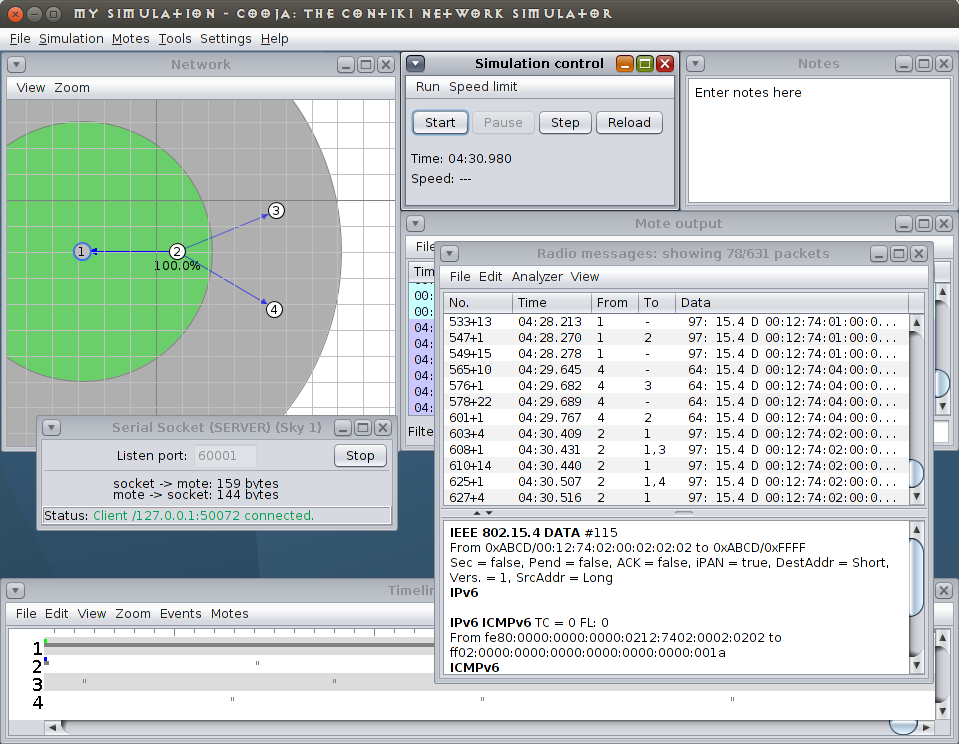
\includegraphics[width=0.8\textwidth]{fig/cooja_example.png}
	\caption{An Example of Cooja Execution}
	\label{Fig: An Example of Cooja Execution}
\end{figure*}

\Cref{Fig: An Example of Cooja Execution} shows a simulation simulating the exact same WSN topology as described in \Cref{Fig: Experiment Setup}, with \textcircled{1} being the Border Router. 

In this project, we are mostly interested in the radio traffic. The traffic is captured by the ``Radio messages'' plugin which exactly serves as the Sniffer in \Cref{Fig: Experiment Setup}. The corresponding pcap file is written by Cooja alongside the simulation under ``cooja/build/'' folder, which can later be opened by Wireshark\cite{Wireshark} for analysis, as shown in \Cref{Fig: A Wireshark Example}.

\begin{figure*}[h!]
	\center
	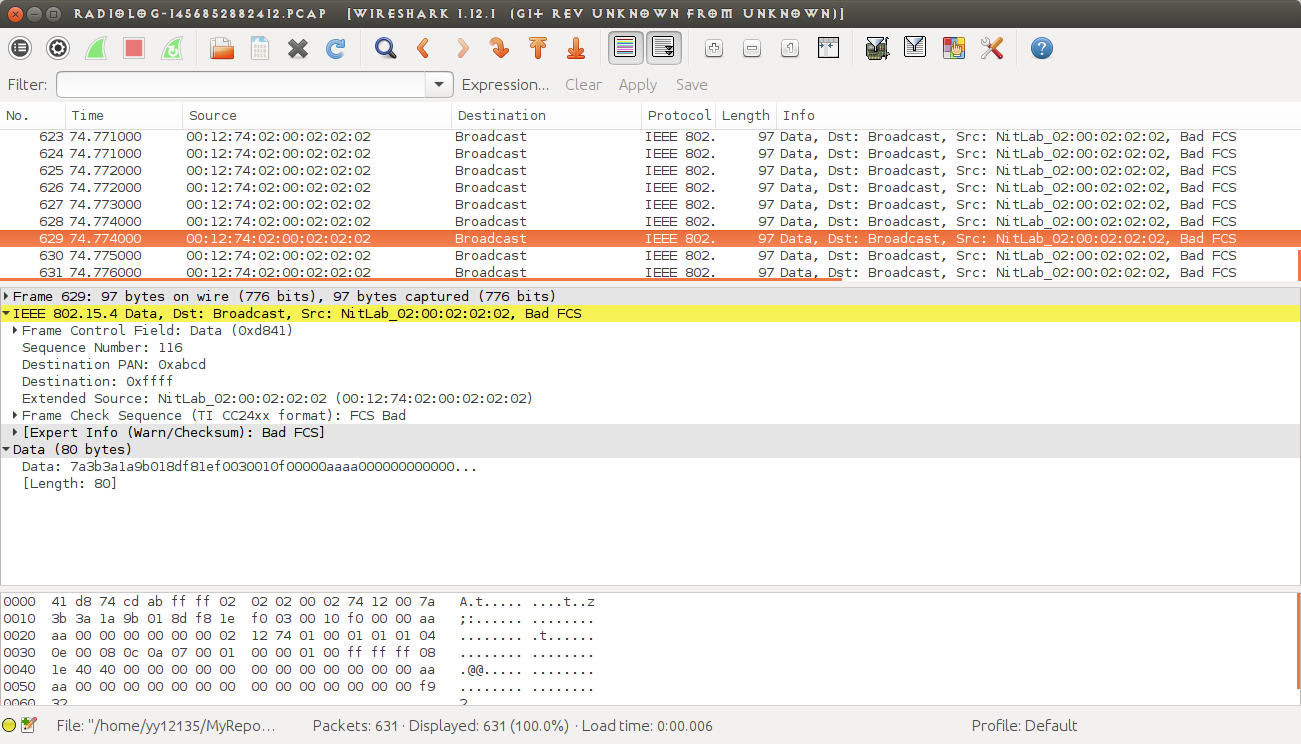
\includegraphics[width=0.8\textwidth]{fig/wireshark_example.png}
	\caption{A Wireshark Example}
	\label{Fig: A Wireshark Example}
\end{figure*}

As of the time of writing this report, Cooja in Contiki release-3.0 supports simulations for TelosB and Wismote. CC2538 is not yet supported in the latest version.

Cooja is not suitable for large scale experiments as there is a potential memory leakage problem which drastically downgrades long time simulations, or sometimes even crashes them. Also notice that the performance of Cooja is obviously better on low performance devices. For example, simulations with TelosB are nearly 8 times efficient than Wismote for the same application code.

\section{Security Measures}

In this report, we analyse traffic that is protected by two security measures implemented on Contiki release-3.0, namely noncoresec and DTLS.

\subsection{noncoresec}

In Contiki source code, LLSEC is an alias for \textit{noncoresec}.

\textit{noncoresec}\cite{noncoresec}\cite{LLSEC} is a reduced 802.15.4 Security implementation on Contiki. \textit{noncoresec} uses a hard coded network shared key that is defined by the ``NONCORESEC\_CONF\_KEY'' macro in ``project-conf.h'' file; thus it cannot be updated during runtime. 

When \textit{noncoresec} is enabled, we always assume it uses the highest Security Level (7), i.e. all frames are encrypted and authenticated in AES-128-CCM* mode with 16 bytes MAC, as described in \Cref{Subsec: 802154 Sec}. With this Security Level, all Sensor Nodes in the WSN must have the same key that is hard coded during compilation. External Sensor Nodes without the key cannot send or receive any frame and thus are repelled from the network.

In scenarios where the WSN is protected by \textit{noncoresec}, we always assume the adversary has no knowledge of the key. This effectively indicates that the adversary is unable to join the network at all since he cannot receive or send any frames as we explained above.

Our code using \textit{noncoresec} are successfully tested on all our devices. However, even though CC2538 has an AES coprocessor built in, the current version of Contiki code does not utilise this feature at all; instead, it uses a textbook software AES implementation as on other platforms. Also notice that the source code of \textit{noncoresec} is only included for TelosB platform by default. When using on other platforms, the developer needs to manually add its source code into the platform specific building system.

\subsection{DTLS} \label{Subsec: Experiment DTLS}

DTLS in Contiki is supported by a third party module \textit{tinydtls}\cite{tinydtls}. \textit{tinydtls} is originally developed for desktop systems and is later ported to Contiki. In the current version tinydtls-0.8.2, there are two cipher suites supported:

\begin{enumerate}
	\item TLS\_ECDHE\_ECDSA\_WITH\_AES\_128\_CCM\_8\cite{rfc7251}
	\item TLS\_PSK\_WITH\_AES\_128\_CCM\_8\cite{rfc6655}
\end{enumerate}

The use of cipher suite can be configured at compiling time by using the ``configure'' script under ``tinydtls-0.8.2'' folder. Also notice that when used with Contiki, ``--with-contiki'' argument is also required when running this script. By default, TLS\_ECDHE\_ECDSA\_WITH\_AES\_128\_CCM\_8 is preferred by the tinydtls implementation.

The keys (or master secrets) can be configured at runtime by using an interface provided by the tinydtls module. When using TLS\_PSK\_WITH\_AES\_128\_CCM\_8, where PSK stands for Pre Shared Key, the same master secrets must be coded beforehand into the clients and servers, or derived by external key management schemes.

The code from the tinydtls official website cannot be directly used on our platforms. The ``tinydtls-0.8.2'' folder in our source code contains a version of code we have tuned for our platforms. When using our code, the following problems should be noticed:

\begin{enumerate}
	\item TelosB does not support tinydtls as the code is oversized and cannot fit into the ROM of this device. Also notice that it cannot transmit frames longer than 127 bytes neither; thus any DTLS handshake message need avoid this type of Sensor Nodes in its path, as packets exceeding this length will be silently dropped by these nodes.
	\item Wismote with TLS\_ECDHE\_ECDSA\_WITH\_AES\_128\_CCM\_8 causes a crash of simulator. We have not yet figure out the exact cause of this problem. A potential cause might be illegal memory access in arithmetic operations.
	\item MTU specified by 802.15.4 Standard is 127 bytes whilst several DTLS handshake messages exceed this limitation. This constriction can be loosen by specifying\\ UIP\_CONF\_BUFFER\_SIZE, QUEUEBUF\_CONF\_NUM and UIP\_CONF\_RECEIVE\_WINDOW macros in ``project-conf.h'' file to a larger value. Nevertheless, specifying larger MTU does not guarantee the success transmission of packets. The handshake packets exceeding 127 bytes would still potentially be silently dropped during runtime.
	\item The handshake packets retransmission should be avoided at best effort. The restransmission implementation of tinydtls should not be relied on as sometimes it is not triggered by a packet lost, potentially due to a signal loss in the Contiki kernel. When a packet is lost during the handshake, the client and server will potentially freeze, resulting into a deadlock. Our current solution is to simply restart the procedure from the beginning, or simply reboot the devices.
	\item TLS\_ECDHE\_ECDSA\_WITH\_AES\_128\_CCM\_8 has a performance issue. Even on CC2538, each curve computation costs roughly 80 seconds on each side. This performance issue somehow triggers other problems in a chain reaction resulting into malfunctioning of the application code. The first problem is that the computation time exceeds the DTLS timeout, which therefore triggers the retransmission problem we described above. We have solved this problem in our code by increasing the timeout. The second problem happens when using  unequal computational power on client and server side, e.g. trying to perform a DTLS handshake from the Laptop through Border Router as the client to a CC2538 Sensor Node in the network. The unequal computational power leads to the fact that the Laptop processes the handshake packets immediately and continuously sends out the responses, without waiting for the Sensor Node to complete its computation. Consequently, the buffer of Sensor Node is instantly over flooded by the handshake packets resulting into some of them being dropped, which, again, triggers the problems caused by retransmission we described above. Our solution to this problem is to simply add a \textit{getchar()} into DTLS client of the Laptop side, of which asks a key stroke before sending each packet
%	\item Multi sessions is not well supported in the current tinydtls implementation on Contiki due to some memory management problem. In another word, try not to establish multiple DTLS sessions with one DTLS server running on the same Sensor Node. Further more, there is a potential memory leakage in tinydtls on termination of a DTLS session, which therefore could potentially crash the application or simulation. 
\item tinydtls is designed with asynchronous I/O. One must carefully designs the application code to use it.
\end{enumerate}

In experiments with DTLS, we consider the adversary is a group of compromised Sensor Nodes in the WSN. In other words, not only having all access to packet transmitted over the network, the adversary is capable to send any crafted packets to any Sensor Node in the network as well. In experiments with TLS\_PSK\_WITH\_AES\_128\_CCM\_8 being the cipher suite, we assume the adversary has no knowledge of the pre shared keys in any other paired Sensor Nodes; otherwise any ciphertext is immediately broken. Similarly, when TLS\_ECDHE\_ECDSA\_WITH\_AES\_128\_CCM\_8 is used, we assume the adversary has no knowledge of the private keys in other Sensor Nodes. In reality, such compromised Sensor Nodes can be Border Routers connected to adversary controlled Laptops deployed among the WSN. .

\subsection{Overloading noncoresec and DTLS}

Theoretically, it is possible to overload noncoresec with DTLS since they are implemented at different layers in the protocol stack. In another word, one can technically use noncoresec to provide MAC Layer security while using DTLS to provide Application Layer security.

However, in Contiki we noticed that either of them de facto adopts AES-128 with CCM mode as the underlining encryption method. Cryptographically speaking, the encryption part of AES-128 with CCM can be viewed as a pseudo random bit stream generator and overloading both of them is equivalent to use another pseudo random bit stream that is the XOR of them. To our knowledge, it is unclear whether this provides more randomness or not. However, intuitively under the assumption that AES-128 can be viewed as a pseudo random function, we argue that this overload does not seem to provide any more confidentiality. The same applies to the CBC-MAC.

On the other hand, the performance impact of overloading cannot be ignored in WSNs. In fact noncoresec and DTLS adds 23 bytes and 21 bytes overhead to each packet respectively whereas the MTU specified by 802.15.4 Standard is only 127 bytes, overloading them will immediately adds great overhead in terms of bandwidth and thus energy consumption. 

Hence, we argue that overloading is not practical and thus is excluded from our experiments.

\section{Applications} \label{Sec: Applications}

In this section we explain some simple applications we have developed in our experiments. These applications are aimed to cover the most generic scenarios of WSN applications. The source code of the applications are located in the ``experiments'' folder in our source code. 

\begin{description}[style=nextline]

	\item[{dtls-telnet}]
	This tool is a DTLS client runs on Linux. It establishes a DTLS session with a DTLS server and runs a telnet application that reads and sends data in ASCII. We use this tool in most of our experiment as the DTLS client. It is located under the ``tools'' folder in our source code.
	
	\item[{dtlsbr}]
	{dtlsbr} is a DTLS echo server merged with a Border Router application running concurrently. An echo server echoes everything received from the clients similar to PING. {dtlsbr} is developed to study how the tinydtls implementation affects the packet features.
	
	\item[{borderest}]
	{boderest} is a CoAP server merged with a Border Router application running concurrently. This application is used to predict some traffic features with CoAPs. Even though there is no security measure adopted in this application, we expect that most of the packet features should be linearly preserved with CoAPs as we explained in \Cref{Subsec: CoAPs}. This application is not compatible with TelosB due to code oversize.
	
	\item[{keydtls}]
	{keydtls} is developed to study how different DTLS session keys affect the packet features. The Sensor Node runs a DTLS server and reads client input, responses with a random string in ASCII representing a sensor reading.
	
	\item[{keyllsec}]
	{keyllsec} is developed to study how different noncoresec keys affect the packet features. There are two sub-applications in this application:
	\begin{itemize}
		\item \textbf{broadcast} application broadcasts an arbitrary message periodically.
		\item \textbf{unicast-sender} and \textbf{unicast-receiver} are a pair of applications where the sender periodically pushes an arbitrary message to the receiver.
	\end{itemize}
	These applications are protected by noncoresec.

	\item[{dtlseiri}]
	\textit{dtlseiri} is developed to study how the execution time of code on a DTLS server affects the time interval of response. Similar to {keydtls}, {dtlseiri} repeatedly calls the Contiki random number generator to generate a random ASCII string as response, representing a sensor reading with additional processing. The execution time is controlled by the number of calls to the random number generator. 

%application detection dtls PINGLOAD
	\item[{dtlspingload}]
	This application is identical to \textit{dtlseiri} but developed for a different purpose. It is used to study a potential side channel attack we named ``pingload'' which we explain in later chapters.
\end{description}

\section{Summary}

In this chapter, we described how our experiments are set up. Two security measures are used in our experiments, namely noncoresec and DTLS. 

We summarise the compatibility of the security measures to the platforms in our experiments as \Cref{Fig: Compatibility of Platforms and Security Measures}.

\begin{table}[h!]
	\center
	\begin{tabular}{|c|c|c|c|}
	\hline
	\multirow{2}{*}{} & \multirow{2}{*}{noncoresec} & \multicolumn{2}{c|}{DTLS} \\ \cline{3-4} 
	                  &                             & ECDHE\_ECDSA & PSK        \\ \hline
	TelosB            & \checkmark                  & N/A          & N/A        \\ \hline
	CC2538            & \checkmark                  & \checkmark   & \checkmark \\ \hline
	Wismote           & \checkmark                  & N/A          & \checkmark \\ \hline
	\end{tabular}
	\caption{Compatibility of Platforms and Security Measures}
	\label{Fig: Compatibility of Platforms and Security Measures}
\end{table}

We have also developed several simple applications to model the most typical WSN application scenarios. We summarize their compatibility in \Cref{Fig: Compatibility of Platforms and Applications}.

\begin{table}[h!]
	\center
	\begin{tabular}{|c|c|c|c|c|c|c|}
	\hline
	\multirow{2}{*}{} & noncoresec & \multicolumn{4}{c|}{DTLS}                           & No Security \\ \cline{2-7} 
	                  & keyllsec   & dtlsbr     & keydtls    & dtlseiri   & dtlspingload & boderest    \\ \hline
	TelosB            & \checkmark & N/A        & N/A        & N/A        & N/A          & N/A         \\ \hline
	CC2538            & \checkmark & \checkmark & \checkmark & \checkmark & \checkmark   & \checkmark  \\ \hline
	Wismote           & \checkmark & \checkmark (*) & \checkmark (*) & \checkmark (*) & \checkmark (*)   & \checkmark  \\ \hline
	\end{tabular}
	\caption{Compatibility of Platforms and Applications}
	\label{Fig: Compatibility of Platforms and Applications}
	(*): As explained in \Cref{Subsec: Experiment DTLS}, on Wismote DTLS can only be used with\\ TLS\_PSK\_AES\_128\_WITH\_CCM\_8.
\end{table}



%A table for available combinations

%\begin{itemize}
%\item{\bf Adversary} is a malicious party that tries to illegally reveal information from the encrypted traffic.
%\item{\bf Border Router}, or BR, is a device that connects adversary to the sensor network. \textbf{BR is not allowed when LLSEC is enabled} as the adversary does not have the key and hence cannot connect into the network. We will discuss more about LLSEC in \Cref{Chp: LLSEC}.
%\item{\bf Sniffer} passively captures all traffic in the network. 
%\item{\bf Target} and {\bf Nodes} are sensors deployed in the sensor network. They communicates to each other through encrypted channels.
%\item{\bf Sensor Network} discussed in this paper is a 6LowPAN network based on Contiki OS.
%\end{itemize}

%Realistically speaking, this scenario could happen say an adversary sitting near a smart house with a laptop attached to a SoC\footnote{System on Chip} device, or your malicious neighbour walks into your smart house with her smart phone.
%
%\section{Adversary Power}
%The powers assumed in the experiments are considered to be practical in real life.
%
%When LLSEC is enabled, all traffic, including RPL\footnote{Routing Procol for Low-power and Lossy Networks} messages, are encrypted; therefore no external nodes can connect to the network as an external node cannot send any valid RPL messages to join the network. The adversary only passively sniffs all traffic.
%
%With LLSEC disabled, the adversary can therefore join the sensor network through a BR and hence is also capable to send messages to the target(s). However, she will not be able to inject any message into an encrypted channel such as a DTLS channel.
%
%\section{Types of Packets}
%We simply categorise the packets into two types:
%\begin{itemize}
%\item {\bf Network Management Packets}: These are the packets generated by the protocols to  maintain the functionality of network, such as MAC ACKs, RPL messages or ICMP messages.
%\item {\bf Data Packets}: These are those packets generated by applications running on sensor nodes., such as a CoAP packet.
%\end{itemize}
%
%This is only a subjective rough categorisation and may not be precise. For example an TCP data packet may set its ACK flag, or DTLS handshake packets could ambiguously fall into both categories. However, we ignore this ambiguity as it is not our focus.